\chapter{AOT 导出：把程序交付为原生产物}
\label{ch:24}

AOT 把经过检查的程序提前编译成目标机器代码。交付时要分别核对编译工具、目标链接资产和应用动态依赖，而不是只检查文件是否已经生成。

\section{运行与导出的配置}

run 默认 checked AOT，适合开发时检查；aot 默认 unchecked，LLVM 优化等级默认为 O3。unchecked 的默认开关主要影响运行期数组与指针检查，不会允许绕过静态所有权或借用规则。

命令选项以 chali help 和 \href{https://github.com/rabbitc999/ChaLi/blob/master/doc/38-aot.md}{LLVM AOT 文档} 为准。不要再使用已删除的 emit 或 .svmb 路径。

\begin{center}
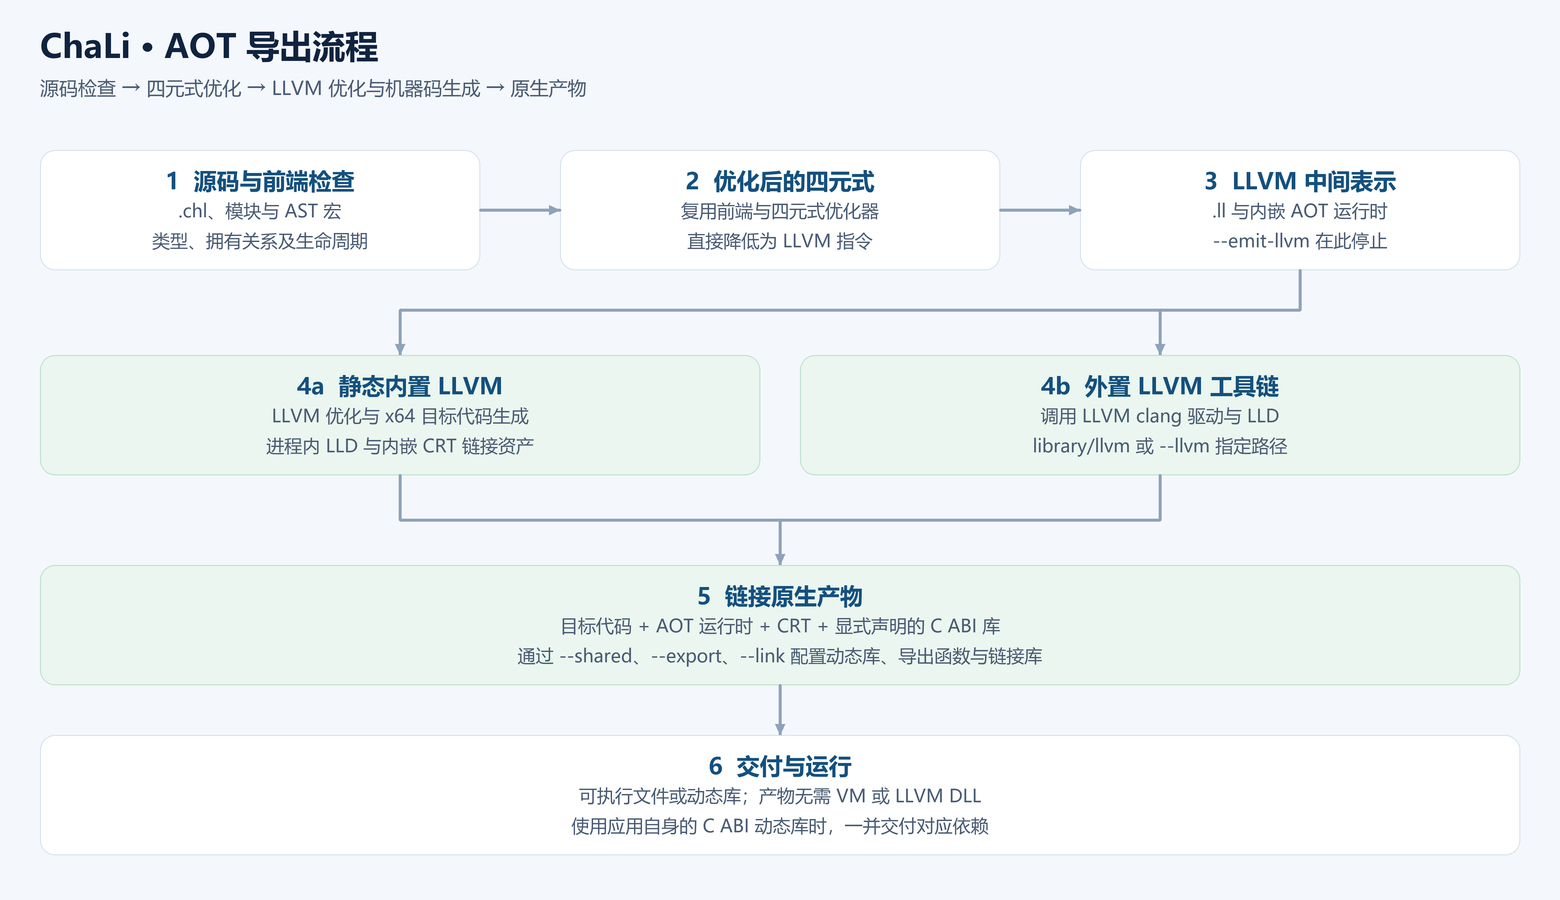
\includegraphics[width=\linewidth,height=0.72\textheight,keepaspectratio]{../images/chali-aot.png}\par
\nopagebreak
AOT 导出与工具链边界
\end{center}

\section{工具链依赖与应用依赖}

内置 LLVM 变体携带编译所需组件，外置变体使用已安装工具链。两者生成的应用按实际链接结果交付；编译器使用 LLVM 不等于应用必须携带 LLVM 动态库。

应用主动调用的 C ABI 动态库、数据库客户端和运行期资源仍按各自约定准备。对最终文件检查真实依赖，不从编译器变体名推断。

\section{交叉编译需要哪些信息}

交叉编译至少要明确目标 triple、CPU／特性、目标 ABI、sysroot、链接器、目标运行库与启动资产。可将受支持配置写入 toml；具体键与命令行覆盖规则按 \href{https://github.com/rabbitc999/ChaLi/blob/master/doc/38-aot.md}{AOT 配置参考} 使用，不把宿主库路径混入目标链接。

\par
\medskip
\begin{lstlisting}[style=cfg]
[aot]
target = "aarch64-unknown-linux-gnu"
cpu = "generic"
sysroot = "build/cross-sdk/linux-arm64/sysroot"
runtime_dir = "build/cross-sdk/linux-arm64/lib"
output = "executable"
\end{lstlisting}
\par
\medskip

\par
\medskip
\begin{lstlisting}[style=sh]
chali aot app.chl --target linux-arm64 --emit-obj --out build/arm64/app
\end{lstlisting}
\par
\medskip

路径相对 chali.toml 解析，命令行显式选项覆盖对应配置。上述 --emit-obj 只生成对象文件，不执行目标链接。

生成某架构对象文件不等于已经得到可部署应用。对象生成、目标链接和目标设备运行需要分别验收；构建出交叉架构编译器也不表示全部 AOT 目标自动可用。

\section{部署核对与诊断}

在干净目录核对配置文件、网页、动态库、数据目录权限及工作目录。首次启动先验证一个无副作用操作，再测试真实业务。需要原生调试时使用 DWARF 与 GDB/MI 路径；保留符号和错误日志，使用户能定位失败阶段。

\section{习题}

\begin{enumerate}

\item 列出编译器依赖与应用依赖各一项。

\item unchecked 是否取消静态借用检查？

\item 跨架构对象生成后还缺什么证据？

\item 部署网页服务时需要带上哪些资源？

\end{enumerate}

\subsection*{参考解答与验收要点}

\begin{enumerate}

\item 例如 LLVM 工具与 MySQL 客户端动态库，按实际链接核对。

\item 不会，默认运行期检查开关与静态规则分别处理。

\item 目标链接与目标环境实际执行。

\item 页面、配置、外部库及数据准备，路径按运行目录检查。

\end{enumerate}

下一章：\hyperref[ch:25]{第 25 章}。

\section{番外：行囊里的工具}

改写自欧阳修《卖油翁》。

陈康肃公善导出，当世无双，公亦以此自矜。尝于家圃编译，有卖油翁释担而立，睨之，久而不去。见其原生产物十发十中，但微颔之。

康肃问曰：“汝亦知 AOT 乎？吾静态 LLVM，不亦精乎？”翁曰：“无他，但工具装得熟尔。”康肃忿然曰：“尔安敢轻吾后端！”

翁曰：“以我酌油知之。”乃取一葫芦，置于地，以钱覆口，徐以杓酌油沥之，自钱孔入，而钱不湿。因曰：“工具在我担中，亦可借隔壁工坊；油入葫芦之后，买油人岂须背着我的油杓回家？”

康肃悟，谓内置 LLVM 是将编译所需工具纳入编译器，外置 LLVM 是借工具链完成同样工序；导出应用不因此平白多带一个 LLVM DLL。

翁将行，又折回道：“不过，若你葫芦上还接着别人家的水管，莫因油杓已收，就说水管也不必交付。”公视之，果有一条自己声明的 C ABI 动态库依赖。

康肃笑而遣之，归来便将发布说明分成工具链依赖与应用依赖两栏。门客称赞文档更长了，公曰：“我宁愿多写两行，也不愿用户半夜来问，油有了，葫芦为什么打不开。”

\subsection*{技术对照}

内置 LLVM 编译器把优化器、代码生成器、链接器和链接资产装进行囊；外置变体借助独立工具链完成这些步骤。交付的原生产物包含所需的 AOT 运行时，应用额外使用的 C ABI 库则按各自的链接约定准备。工具放在哪里与应用依赖哪些库，是两个需要分别核对的问题。
